\setchapterpreamble[u]{\margintoc}
\chapter{Energy System Scenarios}
\labch{ess}

After completing this session successfully, you should be able

\begin{itemize}
    \item to explain what scenarios are and how they are used,
    \item to work with a spreadsheet-based power system model, and
    \item to be able to interpret modelling results.

\end{itemize}


\section{Power sector model}

\paragraph*{Island energy planning and power sector modelling.}
\begin{kaobox}[frametitle=Task]
You have been asked to support local authorities in the planning for a future renewable power system for a remote island. Make yourself familiar with the provided framework of a power sector model together with your course leader.
\end{kaobox}


\section{Scenario analysis}

% TODO: add side note on forecast and weather forecast as example

Models can play various roles when supporting decision-making.  Some, in particular short-term models, can be used to provide \textit{forecasts}, e.g, for the electricity price of the following day. But if decision-makers are interested in long-term strategies as it is mostly the case in energy planning, using models to produce forecast is generally not useful. Planning energy systems usually happens over several decades, with many future uncertainties, from the cost of technologies, to the impact of climate change, to the behaviour of all of us who can shape the future energy system development. Thus, models for energy planning are usually not used to create forecasts, i.e., how the future \textit{will be}, but to create scenarios, i.e., how the future \textit{could be} under certain circumstances. Scenarios are descriptions of potential futures. They can have qualitative elements, i.e., a textual description, and quantitative elements, i.e., a numerical description, for example, graphs. They describe plausible future developments and can help us to explore and think about potential futures. For example, it can support decision-makers in thinking about which might be a preferable energy system and what needs to be done to achieve it.\cite{mcdowall_reflecting_2014}


\begin{kaobox}[frametitle=Shared socioeconomic pathways (SSPs) - Narratives (adopted from \cite{riahi_shared_2017} under CC-BY-4.0), backgroundcolor=Goldenrod!45!white,frametitlebackgroundcolor=Goldenrod!45!white]
\paragraph*{Sustainability – Taking the Green Road.}The world shifts gradually, but pervasively, toward a more sustainable path, emphasizing more inclusive development that respects perceived environmental boundaries. Management of the global commons slowly improves, educational and health investments accelerate the demographic transition, and the emphasis on economic growth shifts toward a broader emphasis on human well-being. Driven by an increasing commitment to achieving development goals, inequality is reduced both across and within countries. Consumption is oriented toward low material growth and lower resource and energy intensity.

\paragraph*{Regional Rivalry – A Rocky Road.}A resurgent nationalism, concerns about competitiveness and security, and regional conflicts push countries to increasingly focus on domestic or, at most, regional issues. Policies shift over time to become increasingly oriented toward national and regional security issues. Countries focus on achieving energy and food security goals within their own regions at the expense of broader-based development. Investments in education and technological development decline. Economic development is slow, consumption is material-intensive, and inequalities persist or worsen over time. Population growth is low in industrialized and high in developing countries. A low international priority for addressing environmental concerns leads to strong environmental degradation in some regions.

\paragraph*{Fossil-fueled Development – Taking the Highway.} This world places increasing faith in competitive markets, innovation and participatory societies to produce rapid technological progress and development of human capital as the path to sustainable development. Global markets are increasingly integrated. There are also strong investments in health, education, and institutions to enhance human and social capital. At the same time, the push for economic and social development is coupled with the exploitation of abundant fossil fuel resources and the adoption of resource and energy intensive lifestyles around the world. All these factors lead to rapid growth of the global economy, while global population peaks and declines in the 21st century. Local environmental problems like air pollution are successfully managed. There is faith in the ability to effectively manage social and ecological systems, including by geo-engineering if necessary.
\end{kaobox}


\begin{figure}[hb]
	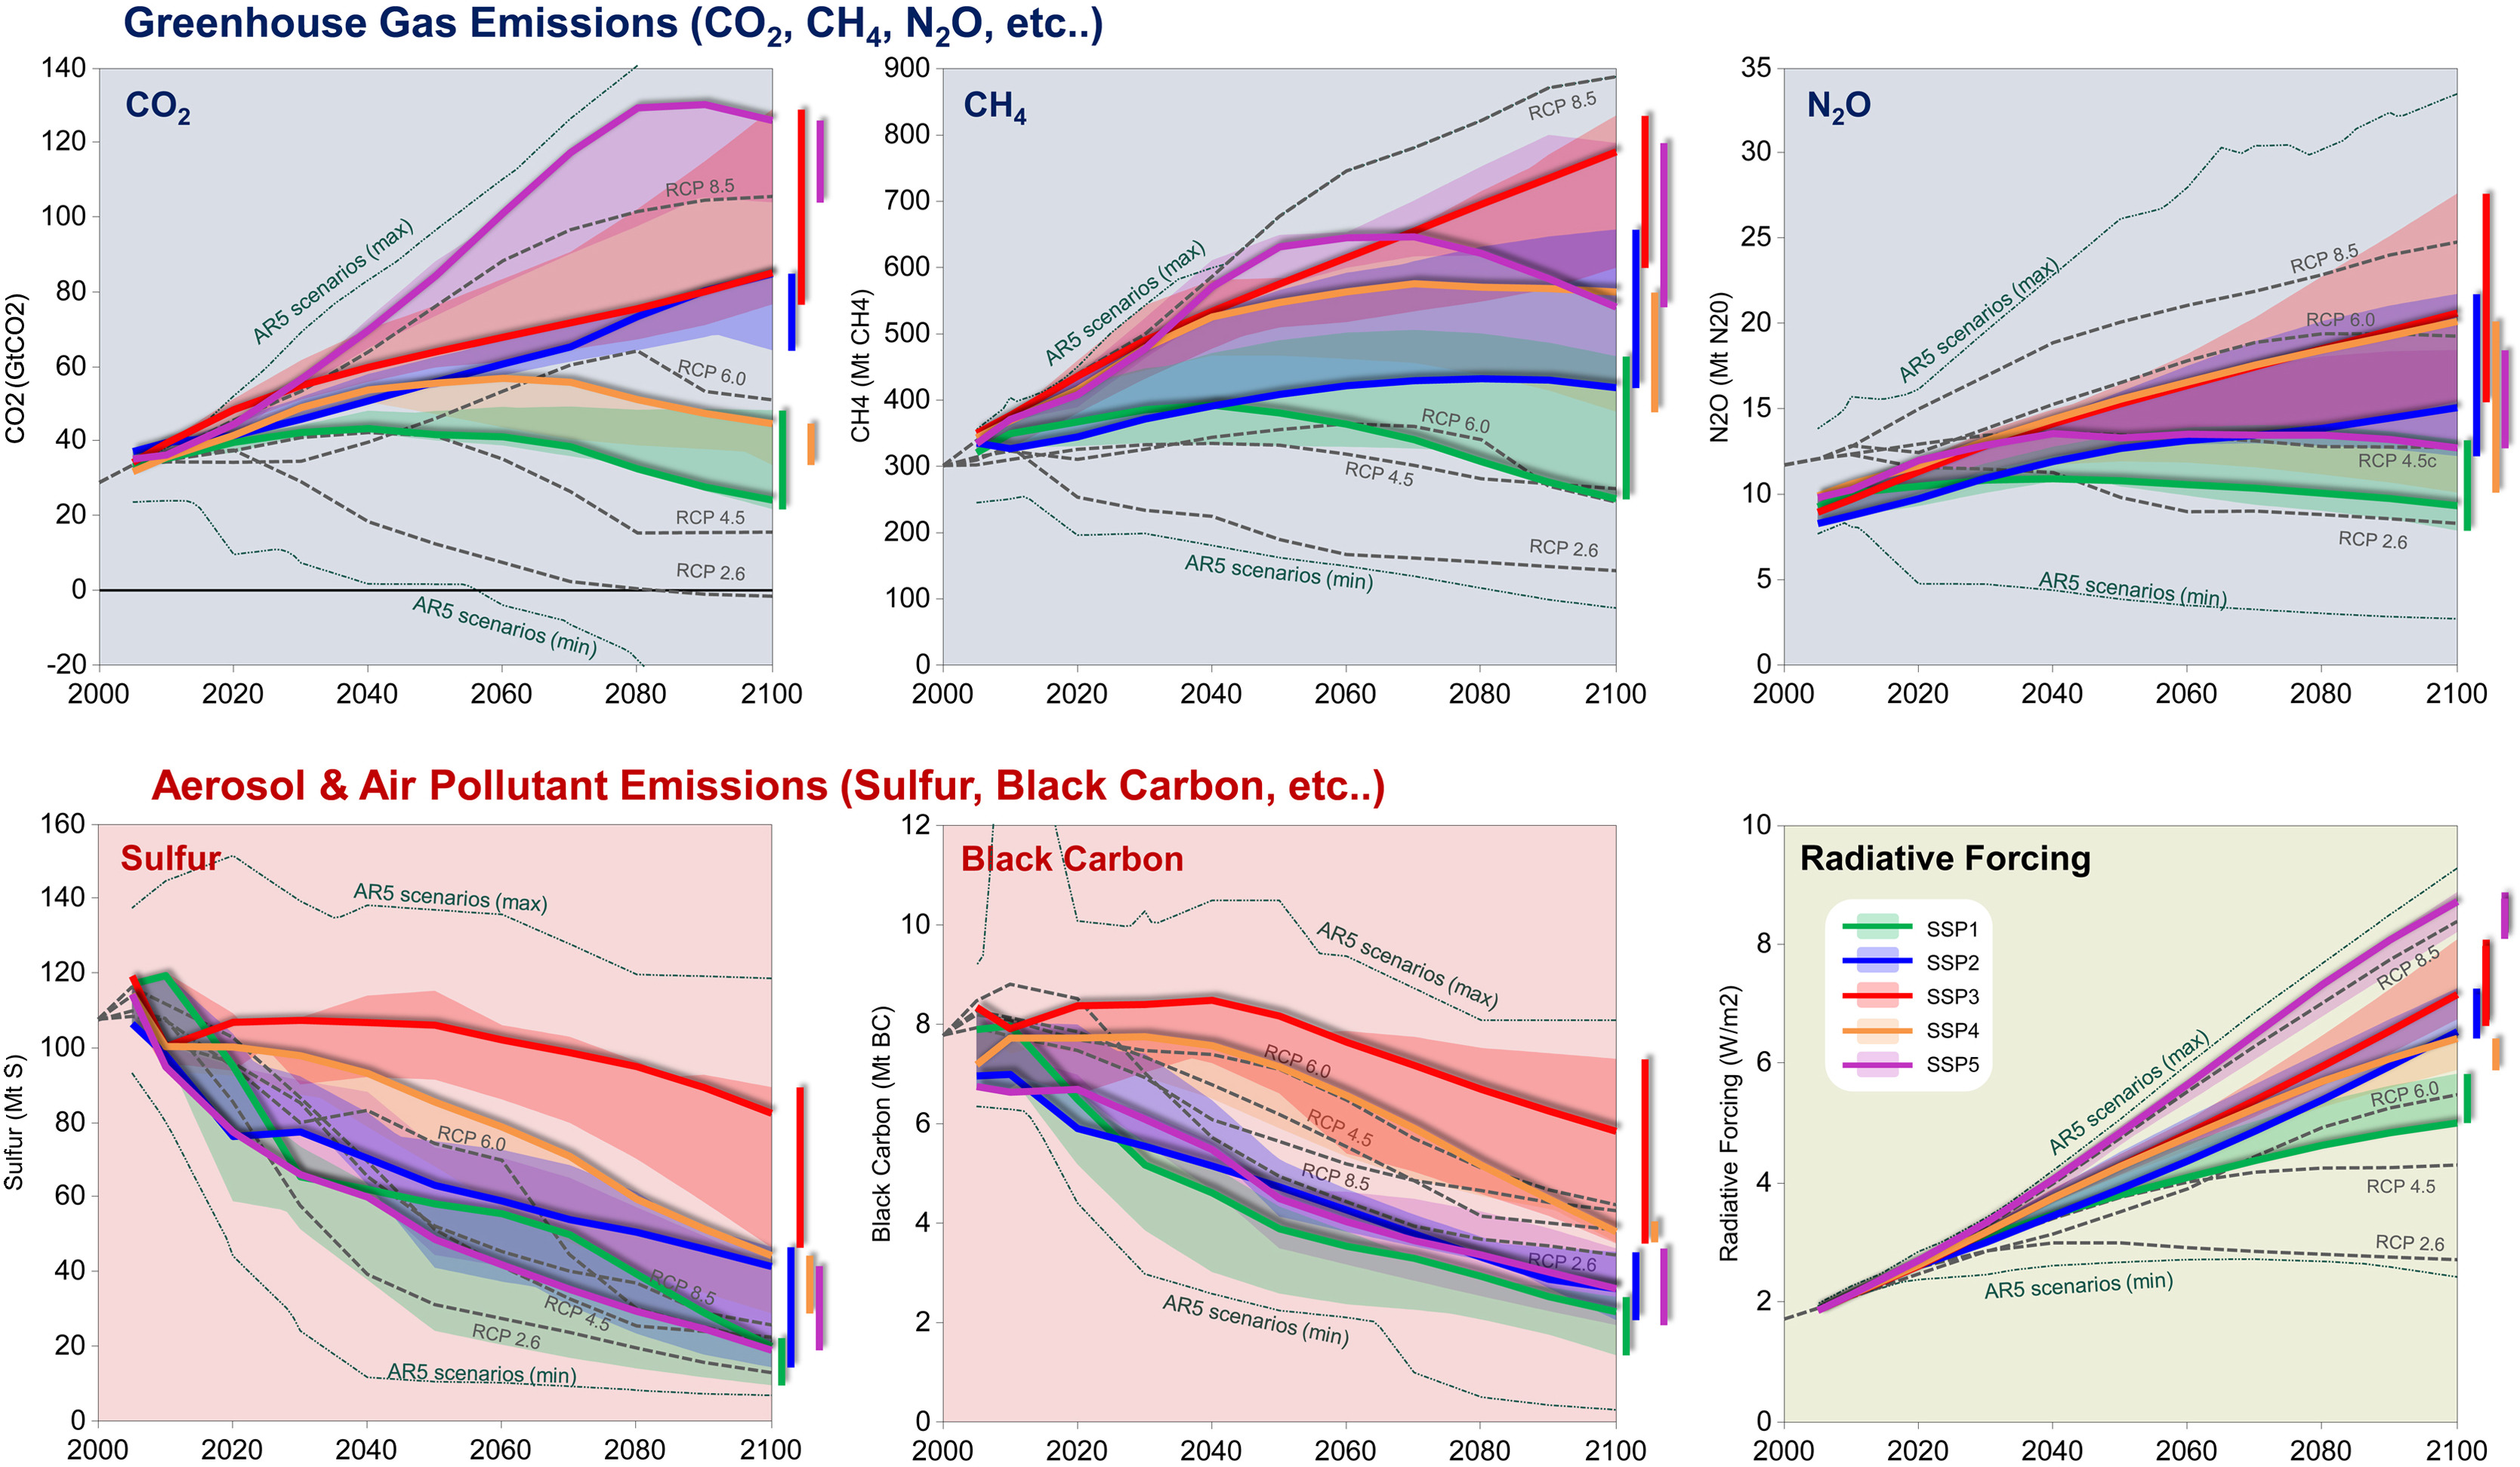
\includegraphics[width=0.98\textwidth]{files/SSP_pathways.jpg}
	\caption[Global emissions and radiative forcing for SSPs.]{Global emissions and radiative forcing for each of the SSPs. Adopted from \cite{riahi_shared_2017} under a CC-BY-4.0 license}
	\labfig{SSP_pathways}
\end{figure}

\begin{kaobox}[frametitle=Task]
Read through the qualitative narratives of the 3 (out of 5) shared socioeconomic pathways above and compare those with the quantitative emission pathways given in \reffig{SSP_pathways}. To which SSP does each of the narrative belong? Explain your choice.
\end{kaobox}


% TODO: potentially add another (optional) exercise for pupils to write one or two scenario for, e.g., the UK or the island system from before




\section{Homework}

\paragraph*{Part 1.} Have a look at and get familiar with the power sector model from the this session which will be provided by your course leader. Use the model to explore one scenario and prepare a 1-2 minute presentation of it for the next session. You can use the data already in the spreadsheet and explore this base scenario or change some of the data. You should prepare
\begin{itemize}
\item a name for the scenario,
\item a short (3-4 sentences) narrative for the scenario,
\item a short explanations of the model results (i.e., what power generation technologies will be used),
\item a short (1-2 sentences) conclusion for local policy-makers (i.e, what does the scenario tell them)
\end{itemize}


You do not need to submit this beforehand (but if you want, you can and your course leader will provide feedback) but, as said above, be prepared to present your scenario to your course leader and fellow students in 1-2 minutes.

\paragraph*{Part 2.} Think about which local area (town, city, small island, etc.) you want to help plan a renewable power system in your final assignment. Your course leader will ask for this in the next session to be able to provide you with the correct data for your power system model.